\documentclass[tikz,border=4pt]{standalone}
% Estilo común de los diagramas de bloques (se usa con \input en cada standalone)
\usepackage[defaultsans,scale=0.92]{lato}
\usepackage{libertinust1math}
\usepackage{xcolor,amsmath}
\usepackage{tikz}
\usetikzlibrary{positioning,arrows.meta,calc,shapes.geometric}
\usepackage{../../notacion}
\definecolor{ctrlazul}{HTML}{1E5AA8}\definecolor{ctrlnoche}{HTML}{14213D}
\definecolor{ctrlcoral}{HTML}{D1495B}\definecolor{ctrlverde}{HTML}{2A9D8F}
\definecolor{ctrlambar}{HTML}{E09F3E}\definecolor{ctrlgris}{HTML}{5C677D}
\definecolor{ctrlvioleta}{HTML}{6C4AB6}\definecolor{ctrlteal}{HTML}{0F7173}
\tikzset{
  >={Stealth[length=2.4mm]}, every node/.style={font=\small},
  bloque/.style={draw=ctrlnoche,fill=ctrlazul!7,thick,rounded corners=1.5pt,minimum height=9mm,minimum width=13mm,inner sep=4pt},
  suma/.style={draw=ctrlnoche,thick,circle,inner sep=0pt,minimum size=6mm},
  senal/.style={->,thick,draw=ctrlnoche},
  rot/.style={font=\footnotesize,text=ctrlgris},
}

\begin{document}
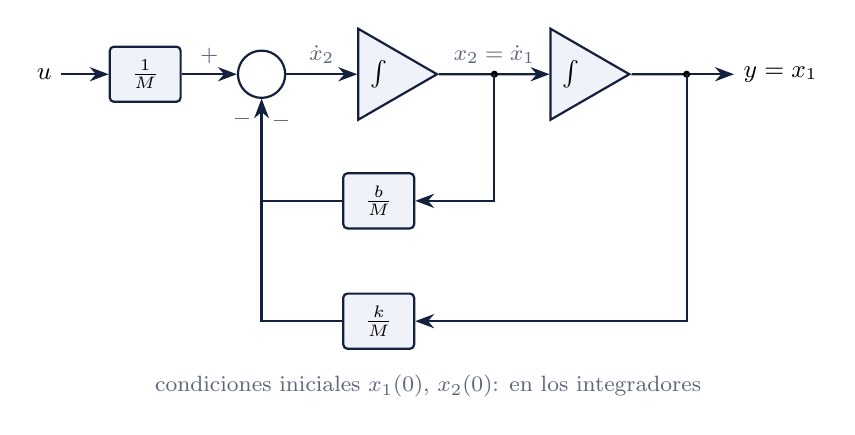
\begin{tikzpicture}[int/.style={draw=ctrlnoche,thick,fill=ctrlazul!7,isosceles triangle,isosceles triangle apex angle=60,minimum size=10mm,inner sep=1pt},
                    gan/.style={bloque,minimum width=9mm,minimum height=7mm}]
  \node (u) {$u$};
  \node[gan,right=6mm of u] (m) {$\frac1M$};
  \node[suma,right=7mm of m] (S) {};
  \node[int,right=9mm of S] (i1) {$\int$};
  \node[int,right=14mm of i1] (i2) {$\int$};
  \coordinate[right=7mm of i2] (o); \node[right=6mm of o] (y) {$y=x_1$};
  \node[gan,below=8mm of i1] (b) {$\frac bM$};
  \node[gan,below=8mm of b] (k) {$\frac kM$};
  \draw[senal] (u)--(m); \draw[senal] (m)--node[above,rot]{$+$}(S);
  \draw[senal] (S)--node[above,rot]{$\dot x_2$}(i1);
  \draw[senal] (i1)--node[above,rot]{$x_2=\dot x_1$}(i2);
  \draw[thick,draw=ctrlnoche] (i2)--(o); \draw[senal] (o)--(y); \fill (o) circle (1.3pt);
  \coordinate (v) at ($(i1.east)!0.5!(i2.west)$); \fill (v) circle (1.3pt);
  \draw[senal] (v)|-(b); \draw[senal] (o)|-(k);
  \draw[senal] (b)-|node[pos=0.9,left,rot]{$-$}(S);
  \draw[senal] (k)-|node[pos=0.95,right,rot]{$-$}(S);
  \node[rot,align=left,anchor=north west] at ($(k.south west)+(-2.5,-0.2)$) {condiciones iniciales $x_1(0)$, $x_2(0)$: en los integradores};
\end{tikzpicture}
\end{document}
